\documentclass{article}

\usepackage[utf8]{inputenc} % allow utf-8 input
\usepackage[T1]{fontenc}    % use 8-bit T1 fonts
\usepackage{hyperref}       % hyperlinks
\usepackage{url}            % simple URL typesetting
\usepackage{booktabs}       % professional-quality tables
\usepackage{amsfonts}       % blackboard math symbols
\usepackage{nicefrac}       % compact symbols for 1/2, etc.
\usepackage{microtype}      % microtypography
\usepackage{lipsum}
\usepackage{graphicx}
\usepackage{amsmath}
\usepackage{upgreek}
\usepackage{tikz}
\usepackage{bm}

\usetikzlibrary{
  arrows.meta, % for Straight Barb arrow tip
  fit, % to fit the group box around the central neurons
  positioning, % for relative positioning of the neurons
}

\title{Blockchain Transmission Protocol: A Brief Introduction}
\author{
  Scott Smiley, Cyrus Vorwald, Eric Solomon, Elise Shin \\
  ICON Foundation \\
  \and
  MoonKyu Song \\
  ICONLOOP \\
}

\newcounter{algo_steps}

\begin{document}
\maketitle
\begin{abstract}
An increasing number of teams are creating and launching their own blockchains, drawn both by the merits of building customized platforms and the increasing ease of doing so. As a result of the growing number of blockchains, there is a need for solutions that connect siloed systems to leverage the various offerings spread across blockchains. 

In response to this trend, various cross-chain messaging protocols have thus far been introduced, characterized by a tradeoff between cost, security, extensibility, and speed. The Blockchain Transmission Protocol (“BTP”) is a chain-agnostic and trustless generic messaging protocol that is designed to minimize this tradeoff with the use of gas-efficient, on-chain light clients. 
\end{abstract}

\section{Introduction}
\label{sec:introduction}
The purpose of BTP is to enable complex cross-chain applications with smart contracts residing on two or more blockchain networks with as few security sacrifices as possible. On-chain light clients (“Verifiers”) deployed on all BTP-enabled blockchains are key components of the BTP architecture designed to achieve this goal. 

While on-chain light clients pose challenges of gas cost and maintenance, the ICON blockchain has been optimized to support this implementation, mitigating the cost of maintenance and providing a secure, cost-efficient, and trustless cross-chain messaging protocol.

This paper provides a summary of the existing solutions in comparison to BTP, the components of BTP, a walk through of the process for integrating those components with a blockchain,\footnote{For more information about the data structures in BTP, visit \url{https://github.com/icon-project/btp/blob/iconloop/doc/icon.md}} and an explanation of the specific modifications made to the ICON blockchain to support this protocol.

\section{Existing Solutions}
\label{sec:relatedwork}
There are several existing models for cross-chain messaging. The following are the most popular solutions as of today:

\textbf{Proof-Of-Authority Consensus} - Rely on signatures by permissioned validators to confirm to the destination chain that a transaction occurred on the source chain. Because validators are assumed to be trustworthy, verification is unnecessary.
Example Implementation: Wormhole \cite{wormhole}

\textbf{SMPC (Secure-Multiparty-Computation)} - Securely and secretly break a private key into many pieces, then distribute the pieces amongst a validator set. The validator set can be permissioned (i.e. Proof of Authority) or permissionless (i.e. Proof of Stake). Validators form consensus on transactions that occur on the source chain and relay transactions deemed valid to the destination chain.
Example Implementation: MultiChain~\cite{multichain}

\textbf{Relay + Oracle} - Rely on two-party consensus between a Relay with message proofs and an Oracle to provide block data. The transaction proof is checked against the block data to validate its authenticity.
Example Implementation: LayerZero~\cite{layerzero}

\textbf{Optimistic Interchain Communication} - Assume all transactions are honest, usually after a certain time frame, and rely on off-chain participants to report malicious activity. Malicious activity is easily detectable by design. It can be accompanied with Proof of Stake to punish malicious participants.
Example Implementation: Optics~\cite{optics}, Nomad~\cite{nomad}

\textbf{Light Client} - Rely on a light-client to validate data from a source blockchain on the destination blockchain. A Relay forwards message proofs from the source to the destination, where the destination has a light client of the source to validate the message proof.
Example Implementation: IBC~\cite{cosmos}

\section{BTP Security Model}
\label{chap:overview}
BTP leverages light clients for on-chain verification of messages passed between blockchains. There are two common challenges with light client solutions:

\begin{enumerate}
\item Extensibility - Integrating new networks can be difficult and time consuming
\item Maintenance costs - Updating on-chain light clients with live block data can be prohibitively expensive
\end{enumerate}

BTP addresses both of the aforementioned challenges. Extensibility, in the context of integrating new networks to the BTP ecosystem, is achieved through the use of on-chain light clients and a hub architecture. The hub architecture refers to a blockchain that is used as an intermediary to route messages from the source blockchain to the destination blockchain. More details on the ICON blockchain architecture that enables it to efficiently operate as a hub can be found in the section titled \textit{\nameref{modifications}}.

The hub model includes light clients of all connected networks deployed on one network. It also makes new integrations easier. The hub maintains light clients of all connected networks to verify and route transactions as needed. New integrations must only deploy the light client of the hub, which can be easily copied or translated from existing implementations. See \ref{fig:hub} below for a graphical depiction of the hub architecture.


\begin{figure}[!ht]
\begin{center}
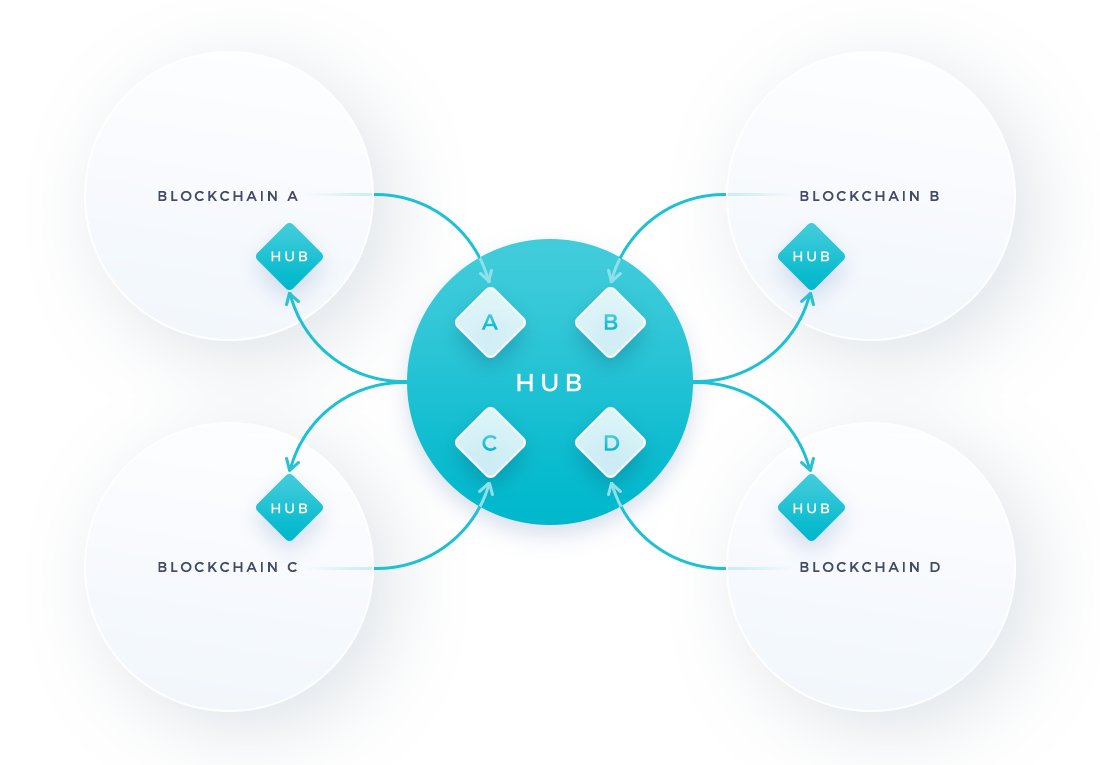
\includegraphics[width=12cm]{./images/Hub.png}
\caption{Hub architecture}
\label{fig:hub}
\end{center}
\end{figure}

Existing light client solutions may require the target blockchain’s validators to upgrade their software, which calls for a network hard-fork. On-chain light clients remove this requirement because the light client state is deployed and maintained at the smart contract layer. This makes it easier to deploy BTP to new networks, because neither permission nor action is required from the target network.

Maintenance costs are addressed by two features on the core ICON blockchain: BTP Blocks and the Verifier Whitelist. See the section titled \textit{\nameref{modifications}} for more information on how maintenance costs are addressed using these features.


\section{Components}
\label{sec:components}

BTP includes one off-chain component as well as a set of smart contracts to process and verify messages (the reason for the off-chain component is explained in the component subsection titled \textit{\nameref{relay}}.):

\begin{enumerate}
\item Service Handler
\item Message Broker
\item Message Relay (off-chain)
\item Message Verifier
\end{enumerate}

For more information about the components, visit \url{https://github.com/icon-project/IIPs/blob/master/IIPS/iip-25.md}

\subsection{Service Handler}
The service handler handles requests to send any instructions from one blockchain to another. Only permissioned Service Handlers may call a Broker (described in the next section) in order to prevent malicious contracts from attacking the BTP network.

The primary service handler is the Arbitrary Call Service, which allows for third-party developers to build their own bespoke services as extensions of BTP. End users will call the Service Handler on the source blockchain, resulting in a BTP message being sent to the destination blockchain. \textit{Depending on an application developer’s design decisions, users may need to call functions to execute the transaction on the destination network.}

\subsection{Message Broker}
Message brokers, which may be shortened to brokers, act as central hubs of all BTP messages for their respective networks. Each BTP-enabled network has one message broker smart contract at minimum – however, it can have more to scale with the number of messages if needed.

The message broker links the permissioned service handler and message verifier. On the sending blockchain, the message broker translates service messages from the service handler to BTP messages and sequentially routes BTP messages to the message relay. On the receiving blockchain, the message broker sequentially routes all relay messages to the message verifier and sequentially routes verified BTP messages to the service handler.

\subsection{Message Relay}
\label{relay}
The relay, short for message relay, is a necessary off-chain component because blockchain networks are inherently restricted from initiating outward calls to external networks. In the context of BTP, a relay is defined as an incentivized off-chain server that forwards messages and synchronizes the message verifiers between blockchains.

Relay messages are Recursive Length Prefix (RLP)-encoded BTP messages that include block updates, block proofs, and message proofs.\cite{rlp} All relay messages are delivered in order, using a sequence number that prevents skipped or duplicated messages.\footnote{For more information about the relay message data structure, visit \url{https://github.com/icon-project/btp/blob/iconloop/doc/icon.md\#relaymessage}}

\subsection{Message Verifier}

The message verifier is an on-chain light client of the source blockchain, stored in a smart contract on the destination blockchain. It sequentially decodes and verifies relay messages using block headers and validator signatures from the source blockchain.

Message verifiers track block headers, as opposed to full blocks, and receive block updates from message relays to arrive at the latest state. This state is typically the merkle root of the old block headers. With this information, the message verifier can prove inclusion of a given block header using only the security assumptions of the source blockchain.

\section{Integration of Components}
This section will walk through an example transaction of sending a BTP-enabled token from Blockchain A to Blockchain B using the Arbitrary Call Service and each of the aforementioned components.

\subsection{Arbitrary Call Service}
The following example uses the Arbitrary Call Service to enable a proof of concept of a “BTP Token.” A wrapped token is collateralized by native tokens on the source blockchain locked in a smart contract awaiting redemption, while a BTP token has mint and burn permissions triggered by BTP Messages as illustrated below. Note that certain transactions should be able to be reverted in the event of cross chain message failure. For a BTP token, this means refunding burned tokens if the cross-chain transaction fails.

\subsection{Example}

\begin{figure}[!ht]
\begin{center}
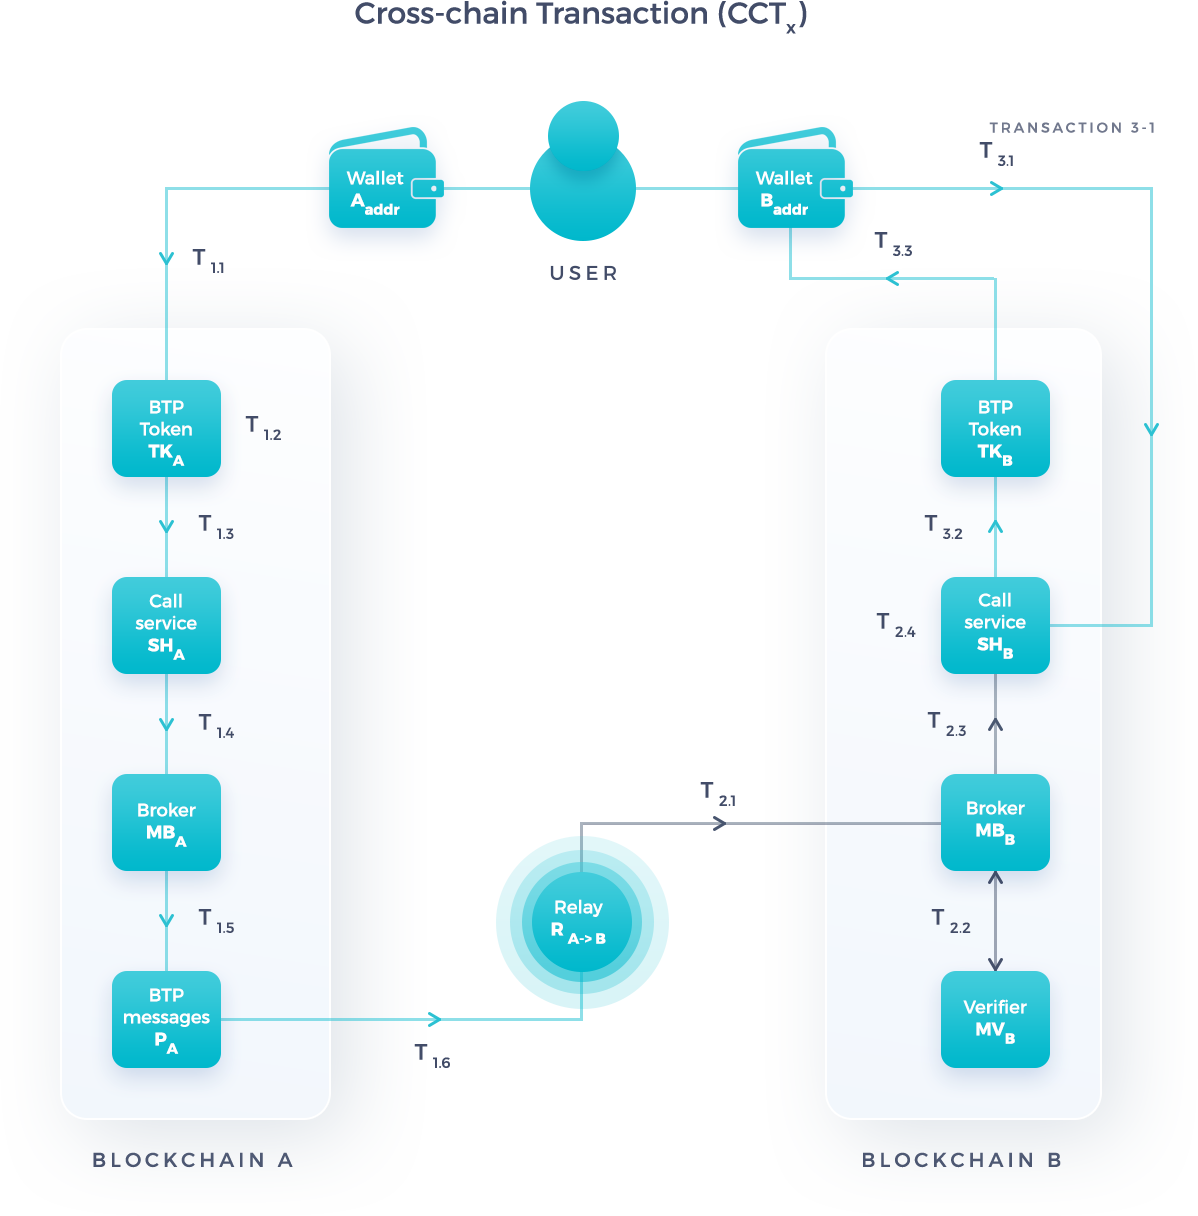
\includegraphics[width=12cm]{./images/Cross-chain Transaction.png}
\caption{Cross-chain transaction}
\label{fig:cct}
\end{center}
\end{figure}
{\setlength{\parindent}{0cm}{
Let's say a user wants to perform cross chain transaction $CCT_x$ to transfer $x$ amount of BTP-enabled token $TK$\footnote{A BTP-enabled token transfers tokens across blockchains by burning tokens on the sending blockchain, and minting tokens on the receiving blockchain.} from blockchain $A$ to blockchain $B$. The user's wallet address on $A$ is $A_{addr}$ and the user’s wallet address on $B$ is $B_{addr}$. We represent this transaction as payload $P$ with ordered unique identifier $N$.\\

\textbf{Atomicity}\\
$CCT_x$ consists of 3 on-chain transactions. $CCT_x$ is successful if and only if the following 3 transactions are all successful.\\

\hspace{10pt} $T_1 = A_{addr} - x ; P_A \rightarrow P_R$

\hspace{10pt} $T_2 = P_R -> P_B ; verify(T_1)$

\hspace{10pt} $T_3 = B_{addr} + x$\\

Otherwise, $CCT_x$ is rejected, the process backs out, and $x$ user funds at $A_{addr}$ are intact.\footnote{Note that certain transactions should be able to be reverted in the event of cross chain message failure. For a BTP token, this means refunding burned tokens if the cross-chain transaction fails.}\\

\textbf{{$\bm{T_1}$: Initiated on the source chain by the user}}
\begin{enumerate}
\item User calls $TK_A.send(B_{NID}, B_{addr}, x)$ to initiate $T_1$. $B_{NID}$ is $B$’s network ID.
\item $TK_A$ burns $x TK$ from $A_{addr}$.
\item $TK_A$ calls $SH_A$.sendCallMessage($B_{NID}, P_A, E)$, where $P_A$ is the $CCT_x$ payload on $A$ and $E$ is the rollback function for error handling associated with $TK_A.send$.\footnote{If $\forall(T_1, T_2, T_3)$ fail, a failure message routes to $SH_A$ which calls E to revert A’s state.} $SH_A$ assigns monotonically increasing sequence number $N$ to $P_A$.\footnote{ For simplicity, we assign the service handler’s sequence number to be the same as the message broker’s sequence number. In practice, these parameters are different because there can be many independent service handlers routing to the same message broker.}
\item $SH_A$ calls $MB_A.sendMessage(B_{NID}, SH_{B_ID}, N, P_A)$, where $MB_A$ is the message broker on blockchain $A$, and $SH_{B_ID}$ is the ID of the service handler on blockchain $B$.
\item $MB_A$ emits $P_A$.
\item Relay $R_{A \rightarrow B}$ listens for $P_A$.
\setcounter{algo_steps}{\value{enumi}}
\end{enumerate}
\textbf{$\bm{T2}$: Initiated on the destination chain by $\bm{R_{A \rightarrow B}}$}
\begin{enumerate}
\setcounter{enumi}{\value{algo_steps}}
\item $R_{A \rightarrow B}$ routes $P$ to $MB_B$ via $MB_B.handleRelayMessage(MB_{A_ID}, P_R)$, where $P_R$ is the $CCT_x$ payload RLP encoded and includes merkle proof that $P_A \exists A$.
\item $MB_B$ calls $MV_B.handleRelayMessage(MB_{B_ID}, MB_{A_ID}, N, P_R)$ which decodes and verifies $P_R$.
\item $MB_B$ calls $SH_B.handleBTPMessage(A_{NID}, SH_{B_ID}, N, P_B)$ to trigger $P_B$.
\item$SH_B$ emits $P_B$ to notify the user of $T_2$’s execution.
\setcounter{algo_steps}{\value{enumi}}
\end{enumerate}
\textbf{$\bm{T_3}$: Initiated on the destination chain by the user}\footnote{Note that $T_3$ could be initiated by any account, but in this example it is initiated by the user.}
\begin{enumerate}
\setcounter{enumi}{\value{algo_steps}}
\item User calls $SH_B.executeCall(N)$ to begin the minting process.
\item $SH_B$ calls $TK_B.mint(x, B_{addr})$.
\item $TK_B$ mints $x TK$ to $B_{addr}$.
\end{enumerate}
Note that in this example, $CCT_x$ involves transferring $x$ $TK$ from $A$ to $B$, but it could be a cross chain transaction to do anything supported by smart contract functionality. $f(x) = A_{addr} - x$ and $h(x) = B_{addr} + x$ could be replaced with any other functions, and the rest of the steps are the same.
}
}
\section{ICON Blockchain Modifications}
\label{modifications}

BTP’s light client architecture would typically be prohibitively expensive because proof verification is computationally expensive and every block must be verified to keep track of changes to the validator signature list. Additionally, certain smart contract environments may not support the necessary hashing functions, which would require a network hard fork to support BTP.

However, the ICON blockchain will be modified\footnote{ At time of writing, the ICON Network does not have these modifications in production. All blockchain modifications require consensus of validators using network governance processes.} to reduce these costs and remove the necessity for network hardforks using two key features: BTP blocks and the Verifier Whitelist.

\subsection{BTP Blocks}
While ICON blocks are produced every two seconds regardless of BTP activity, BTP blocks are produced only when a BTP Message is sent. BTP blocks are validated by ICON’s validator set and are verifiable through ICON blocks.

BTP blocks are not technically blocks themselves, but contain many similar properties. For example, all BTP blocks have a header, but the blocks themselves are not signed by ICON validators. The roots of BTP blocks are included in ICON blocks, which are then signed by ICON’s validator set. See Figure \ref{fig:btp_blocks} for a graphical representation of BTP blocks.

There will be separate chains of BTP blocks per target network. For example, BTP blocks for Blockchain 1 would only be produced when a user sends a BTP Message to Blockchain 1, while BTP blocks for Blockchain 2 would only be produced when a user sends a BTP Message to Blockchain 2. 

There are two primary benefits of BTP blocks:\\

\begin{enumerate}
\item \textbf{Hashing Algorithms} - Destination chains do not need to support ICON’s specific cryptographic hashing algorithm. Instead, ICON supports the hashing algorithms of the integrated destination chains.
\item \textbf{Update Frequency} - Verifiers on non-ICON chains only need to be updated when there is a BTP Message directed to that respective chain.
\end{enumerate}


\begin{figure}[!ht]
\begin{center}
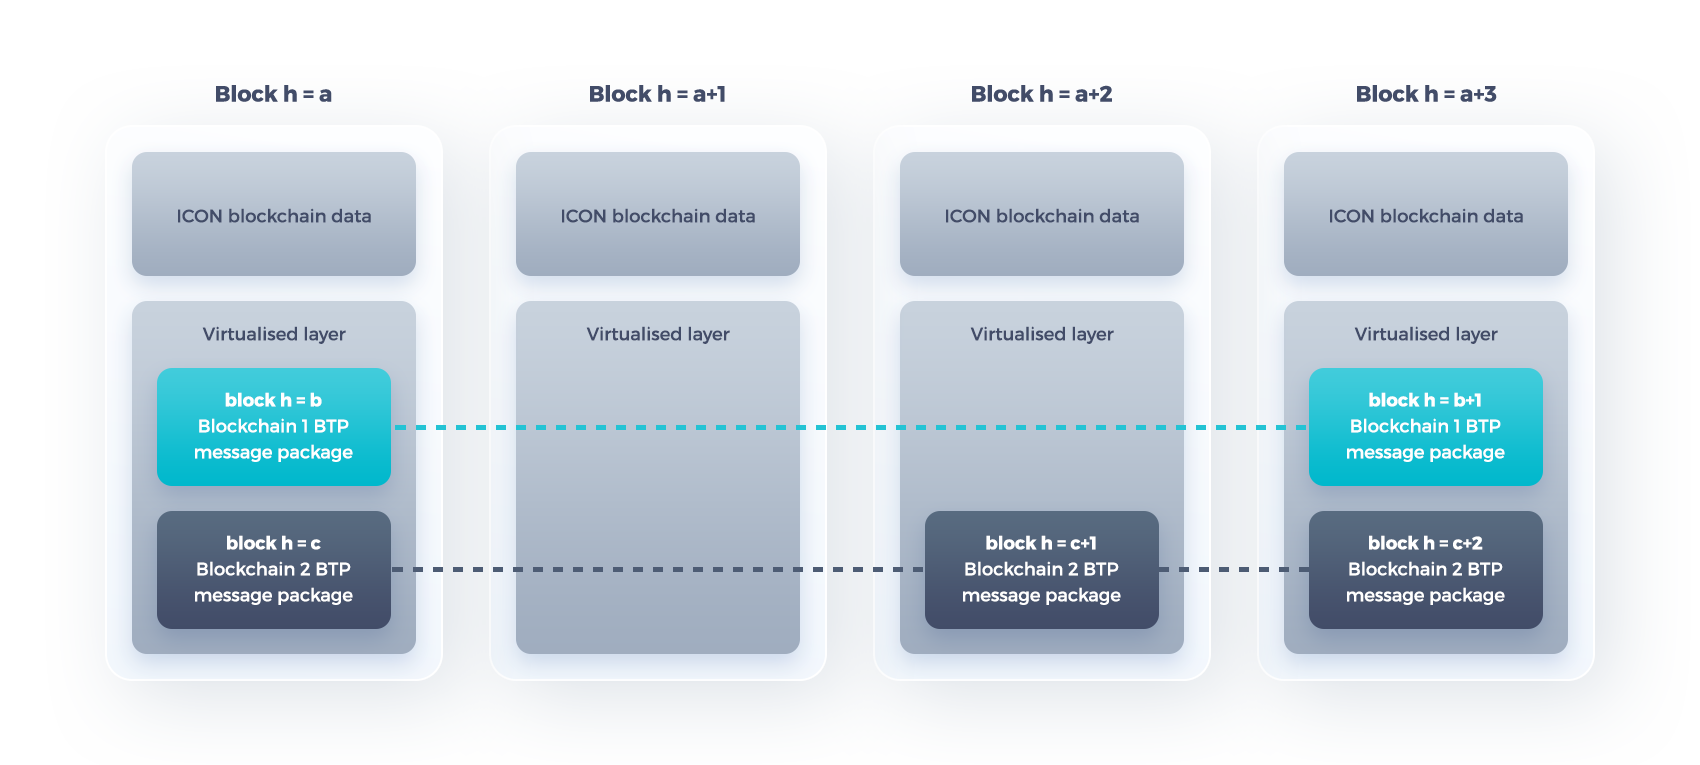
\includegraphics[width=13cm]{./images/BTP.png}
\caption{BTP blocks}
\label{fig:btp_blocks}
\end{center}
\end{figure}

\subsection{Hashing Algorithms}
BTP blocks use cryptographic hashing algorithms that are supported by the smart contract environments of their respective destination chains. For example, BTP blocks with Ethereum as the target network will use the Keccak hashing algorithm since that is what is supported by EVM. Without BTP blocks, ICON would need destination chains to support the SHA3-256 hashing algorithm in their smart contract environments to verify ICON blocks with reasonable gas costs. This often requires a hard fork of the destination chain.

\subsection{Update Frequency}
Message verifiers must receive all blocks in order to maintain their trustless nature. If there is no BTP message in a block, this would result in wasted resources on block update transactions with no relevance to BTP. ICON has 2-second block time, which could lead to many irrelevant block updates.

To solve this issue, the ICON Network has implemented the BTP block as an internal blockchain structure specifically dedicated to validating BTP messages. BTP blocks will not be produced unless there is a BTP message, meaning block updates will only be sent to a non-ICON message verifier when there is a BTP message directed toward that respective network. This results in considerable savings on gas costs.

\subsection{Verifier Whitelist}
ICON-based message verifiers will also require regular block updates from message relays. In order to mitigate the cost for message relays, the ICON Blockchain implements a whitelist for message verifier contracts that will remove the gas costs for all successful block update calls.

In order to monitor the computational resources used by message verifiers, the whitelist still calculates the gas cost of each transaction, but does not apply the fee on successful transactions. This mitigates the cost of maintenance while still monitoring network resource consumption.

An alternative to the Message Verifier Whitelist would be to add the message verifiers as precompiled contracts. This solution, however, would limit the extensibility of BTP and add significant complexity to ICON’s core infrastructure. Adding new precompiled contracts would require a network hard fork when adding a new BTP integration and the message verifiers would need to be written in Go, which is far more difficult than Java, Solidity or Rust.

\section{Conclusion}

Most existing cross-chain messaging protocols rely on trust assumptions to enable practical implementations. This paper proposes a hub-based light client model, in which an intermediary blockchain and an associated off-chain message relay system maintain on-chain light clients of all connected networks and route messages between the source and destination blockchains to enable cross-chain transactions. 

The proposed solution includes the use of an on-chain light client responsible for verifying cross-chain messages. While on-chain light clients pose challenges of gas cost and maintenance, the ICON blockchain has been modified to support the proposed hub model, which mitigates the cost of maintenance and makes BTP the optimal solution for secure, cost-efficient and trustless cross-chain messaging. \\

\textit{Disclosure: The information described in this paper is preliminary and subject to change at any time. Furthermore, this paper may contain “forward-looking statements.”}\footnote{Forward-looking statements generally relate to future events or our future performance. This includes, but is not limited to, ICON’s projected performance; the expected development of its business and projects; execution of its vision and growth strategy; and completion of projects that are currently underway, in development or otherwise under consideration. Forward-looking statements represent our management’s beliefs and assumptions only as of the date of this presentation. These statements are not guarantees of future performance and undue reliance should not be placed on them. Such forward-looking statements necessarily involve known and unknown risks, which may cause actual performance and results in future periods to differ materially from any projections expressed or implied herein. ICON undertakes no obligation to update forward-looking statements. Although forward-looking statements are our best prediction at the time they are made, there can be no assurance that they will prove to be accurate, as actual results and future events could differ materially. The reader is cautioned not to place undue reliance on forward-looking statements.}

\bibliographystyle{unsrt}  

\begin{thebibliography}{1}

\bibitem{wormhole}
What is Wormhole?, \url{https://docs.wormholenetwork.com/wormhole/}

\bibitem{multichain}
Multichain introduction, \url{https://docs.multichain.org/getting-started/introduction}

\bibitem{layerzero}
What is LayerZero, \url{https://layerzero.gitbook.io/docs/}

\bibitem{optics}
Optics, \url{https://docs.celo.org/celo-codebase/protocol/optics}

\bibitem{nomad}
What is the Nomad Protocol?, \url{https://docs.nomad.xyz/}

\bibitem{cosmos}
High-level Overview, \url{https://docs.cosmos.network}

\bibitem{rlp}
RLP, \url{https://eth.wiki/fundamentals/rlp}

\end{thebibliography}

\end{document}
